\documentclass{beamer}
\usetheme{CambridgeUS}
\DeclareGraphicsExtensions{.pdf, .jpg, .gif, .bmp}
\usepackage{amsmath,amsthm}
%\usepackage[numbers]{natbib}
\usepackage{graphicx}
\usepackage{hyperref}
%\def\newblock{} %this is needed for natbib
\newcommand{\var}{\mathrm{var}}
\newcommand{\cov}{\mathrm{cov}}
\newcommand{\E}{\mathbb{E}}
\newcommand{\N}{\mathcal{N}}
\newcommand{\law}{\overset{D}{\rightarrow}}
\newcommand{\prob}{\overset{P}{\rightarrow}}

%\newtheorem{proposition}{Proposition}
%\newtheorem{theorem}{Theorem}

\begin{document}
\title[Two-Sample Kernel Tests]{Two-Sample Kernel Based Tests}
\author[N. Ray with S. Holmes]{Nelson Ray (joint work with Susan
  Holmes)}
\institute[Stanford]{Stanford University}
\date{February 24, 2012}

\begin{frame}
  \titlepage
\end{frame}

\begin{frame}{Outline}
  \begin{enumerate}
  \item The two-sample problem \pause
  \item Friedman's two-sample test \cite{friedman30908multivariate}:
    leverage regression and classification techniques \pause
  \item Univariate data and linear scoring functions: permutation
    $t$-test \pause
  \item Twitter example for text data \pause
  \item Image data: airplanes and cars / pigeons and roosters
  \end{enumerate}
\end{frame}

\begin{frame}{The Two-Sample Problem}
  \begin{block}{Problem}
      $\{\mathbf{x}_i\}_1^N$ from $p(\mathbf{x})$ and
      $\{\mathbf{z}_i\}_1^M$ from $q(\mathbf{z})$ testing
      $\mathcal{H}_A$: $p \neq q$ against $\mathcal{H}_0$: $p = q$ \pause
  \end{block}

  \begin{block}{Solutions}
      \begin{description}[Two-Sample Tests]
      \item[1D/parametric/shift] $t$-test \pause
      \item[1D/non-parametric/shift] randomization test \pause
      \item[pD/parametric/shift] Hotelling's $T^2$-test \pause
      \item[1D/non-parametric/omnibus] Mann-Whitney U/Wilcoxon
        rank-sum test \pause
      \item[pD/non-parametric/omnibus] Friedman-Rafsky test \pause
      \item[ker/non-parametric/omnibus] KMMD test
  \end{description}
  \end{block}
\end{frame}

\begin{frame}{Friedman's Two-Sample Test}
  \begin{enumerate}
  \item Pool the two samples $\{\mathbf{u}_i\}_1^{N+M} =
    \{\mathbf{x}_i\}_1^{N} \cup \{\mathbf{z}_i\}_1^{M}$. \pause
  \item Assign label $y_i = 1$ to the first group and $y_i = -1$ to
    the second group. \pause
  \item Apply a binary classification learning machine $f$ to the training
    data to score the observations $\{s_i =
    f(\mathbf{u}_i)\}_1^{N+M}$. \pause
  \item Calculate a univariate two-sample test statistic $T =
    T(\{s_i\}_1^N,\{s_i\}_{N+1}^{N+M})$. \pause
  \item Determine the permutation null distribution of the above
    statistic to yield a p-value.
  \end{enumerate}  
\end{frame}

\begin{frame}{Permutation t-test Connection}
  With univariate data and linear scoring functions, Friedman's test reduces
  to the permutation $t$-test.  \pause
  \newline
  \newline 
  With multivariate data, the test is close to Hotelling's
  $T^2$-test.
\end{frame}

\begin{frame}{Warm-up (1D)}
  $x_i \sim \mathcal{N}(0,1), z_i \sim \mathcal{N}(3,1),
  \{u_i\}_{i=1}^{20} = \{x_i\}_1^{10} \cup \{z_i\}_1^{10}$ \pause

  $\hat{f}(u_i) = \hat{\beta}_0 + \hat{\beta}_1 u_i$ \pause

  $|T(\{u_i\}_1^N,\{u_i\}_{N+1}^{N+M})| = 6.12 = |T(\{s_i\}_1^N,\{s_i\}_{N+1}^{N+M})|$
  \begin{figure}
   \centering
   \includegraphics[scale=.3]{1D.png}
 \end{figure}  
\end{frame}

\begin{frame}{Twitter Example}
  \begin{figure}[!ht]
   \centering
   \includegraphics[scale=.3]{pres3.png}
   \includegraphics[scale=.3]{pres4.png}  
 \end{figure}
\end{frame}

\begin{frame}[fragile]{Twitter Data}
  Raw: 
\begin{verbatim}
"BarackObama: We need to reward education reforms that are 
driven not by Washington, but by principals and teachers and
parents. http://OFA.BO/6p2EMy"
"SarahPalinUSA: You betcha!! MT \"@AlaskaAces: Alaska Aces 
are 2011 Kelly Cup Champs w/ 5-3 win over Kalamazoo Wings! 
Aces win  ECHL Championship series 4-1\""
\end{verbatim}
  After pre-processing:
\begin{verbatim}
"we need to reward education reforms that are driven not by 
washington but by principals and teachers and parents "
"you betcha mt alaskaaces alaska aces are  kelly cup champs 
w  win over kalamazoo wings aces win  echl championship 
series "
\end{verbatim}
\end{frame}

\begin{frame}{The Spectrum Kernel}
  Compares two strings based on the their length $k$ contiguous
  subsequences. \pause
  \begin{itemize}
  \item $\mathcal{X}$ is our input space, built up from an alphabet
    $\mathcal{A} = \{a,b,\ldots,z,$ $\}$ with $|\mathcal{A}|=27$. \pause
  \item The $k$-spectrum ($k \geq 1$) of an input sequence is the set
    of all length $k$ contiguous subsequences it contains. \pause
  \item Define the feature map from $\mathcal{X}$ to
    $\mathbb{R}^{|\mathcal{A}|^k}$ by $\Phi_k(x) = (\phi_a(x))_{a \in
      \mathcal{A}^k}$ where $\phi_a(x)$ is the number of times $a$
    occurs in $x$: $\{\#aaa,\#aab,\#aac,\ldots,\}$. \pause
  \item $K_k(x,y) = \langle \Phi_k(x),\Phi_k(y) \rangle$.
  \end{itemize}
\end{frame}

\begin{frame}{Support Vector Machines for Regression}
  $$
  f(x) = \sum_{m=1}^M \beta_m h_m(x) + \beta_0, \quad {h_m(x)} \:
\text{basis functions}
  $$
  \pause 
  To estimate $\beta$ and $\beta_0$, minimize
  $$
  H(\beta,\beta_0) = \sum_{i=1}^N V(y_i-f(x_i)) +
  \frac{\lambda}{2}\sum_{m=1}^M \beta_m^2.
  $$
  \pause
  $V$ is taken to be $\epsilon$-insensitive loss:
  \[
  V_\epsilon(r) = \left\{ 
    \begin{array}{l l}
      0 & \quad \text{if } |r| < \epsilon,\\
      |r|-\epsilon & \quad \text{otherwise.}\\
    \end{array} \right.
  \]
  \pause
  The solution has the form $\hat{f}(x)=\sum_{i=1}^N \hat\alpha_i
  K(x,x_i)$, where $K(x,y)=\langle h(x),h(y) \rangle$.
\end{frame}

\begin{frame}{Twitter Example}
  $p < .001$:
    \begin{figure}[!ht]
   \centering
   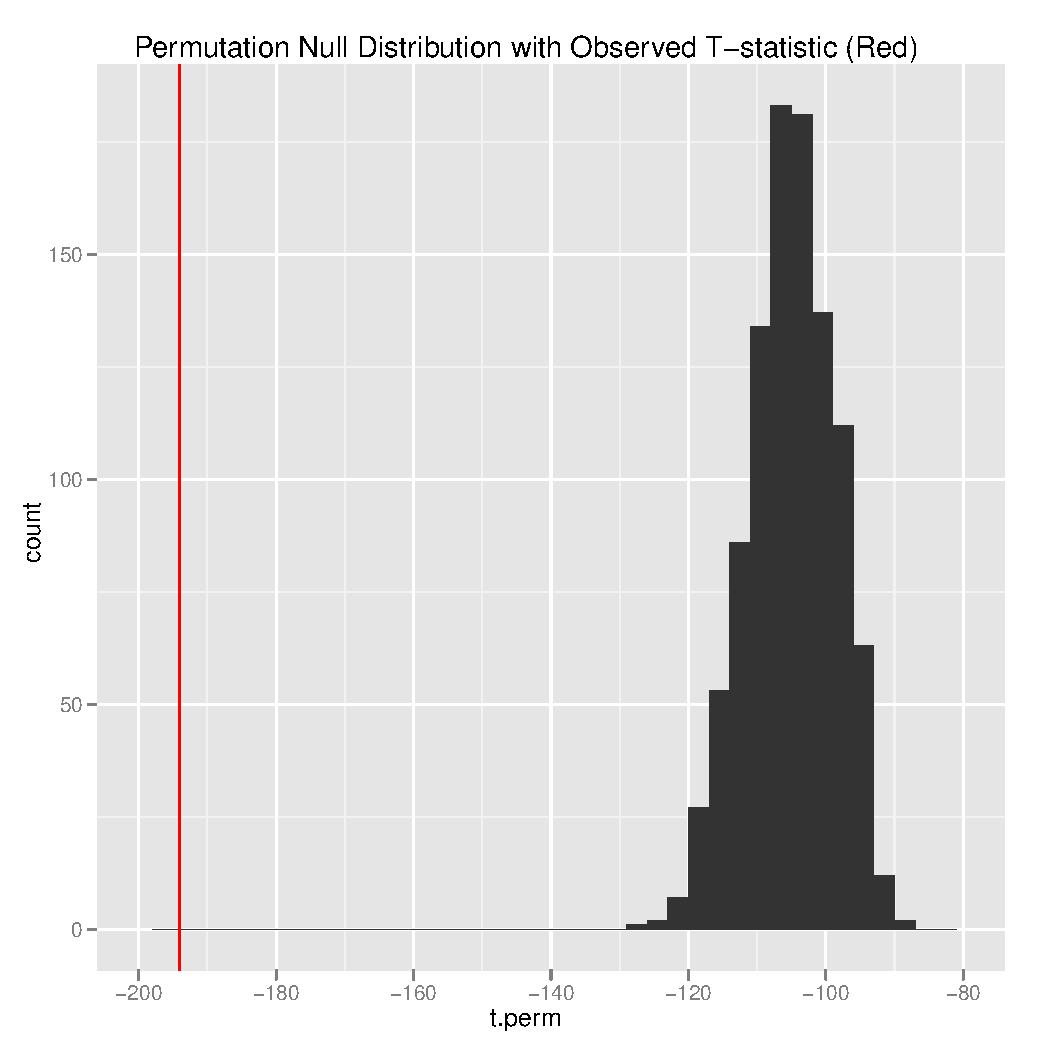
\includegraphics[scale=.4]{pres6.pdf}  
 \end{figure}
\end{frame}

\begin{frame}{Power Simulations at .05 Level}
   \begin{figure}[!ht]
   \centering
   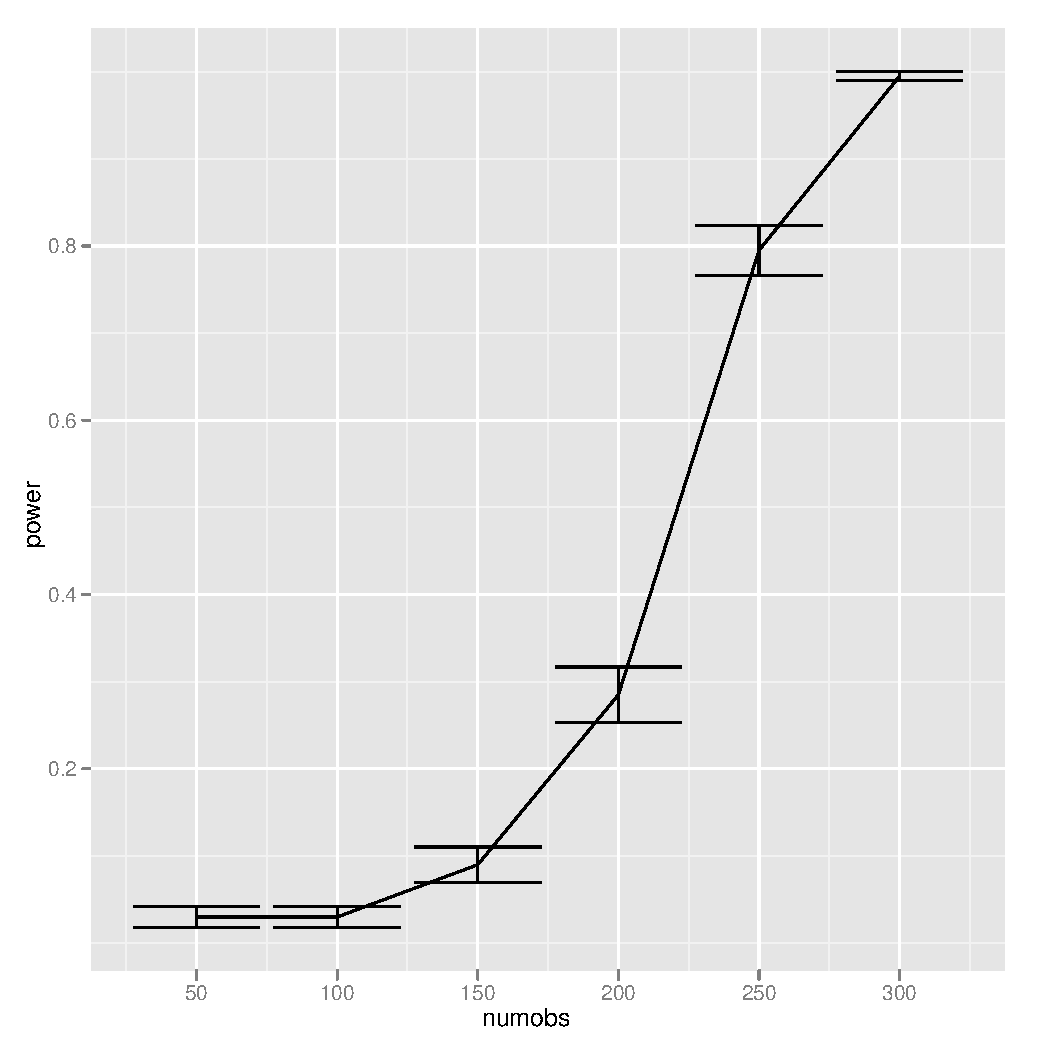
\includegraphics[scale=.4]{pres7.pdf}  
 \end{figure}
\end{frame}

\begin{frame}{Image Data (Cars)}
  Caltech 101 Object Categories \cite{fei2007learning} \\
  The cars are $300\times 197$ grayscale.
  \begin{figure}[!ht]
    \centering
    \includegraphics[scale=.4]{car-image_0001.jpg}
    \includegraphics[scale=.4]{car-image_0002.jpg} \\
    \includegraphics[scale=.4]{car-image_0003.jpg}
    \includegraphics[scale=.4]{car-image_0004.jpg}
  \end{figure}
\end{frame}

\begin{frame}{Planes Before}
  The planes aren't.
  \begin{figure}
    \centering
    \includegraphics[scale=.4]{airplane-image_0001.jpg}
    \includegraphics[scale=.4]{airplane-image_0002.jpg} \\
    \includegraphics[scale=.4]{airplane-image_0003.jpg}
    \includegraphics[scale=.4]{airplane-image_0004.jpg}
  \end{figure}
\end{frame}

\begin{frame}{Planes After}
  \begin{figure}
    \centering
    \includegraphics[scale=.4]{airplaners-image_0001.jpg}
    \includegraphics[scale=.4]{airplaners-image_0002.jpg} \\
    \includegraphics[scale=.4]{airplaners-image_0003.jpg}
    \includegraphics[scale=.4]{airplaners-image_0004.jpg}
  \end{figure}
\end{frame}

\begin{frame}{Polynomial Kernel}
  Each $m \times n$ grayscale image is converted to a vector of
  length $p=mn$.  \pause
  Given $X \in \mathbb{R}^{n \times p}$, the linear kernel is given by
  $$
  K(x, x') = \langle x, x'\rangle = \langle \Phi(x), \Phi(x')\rangle.
  $$
  The kernel matrix is given simply by $XX^T  \succeq 0$.  This
  corresponds to the identity mapping: $\Phi(x) = x$. \pause

  The homogeneous polynomial kernel,
  $$
  K(x, x') = \langle \Phi(x), \Phi(x')\rangle = \langle x, x' \rangle^d, 
  $$
  corresponds to the mapping $\Phi(x) = [x_1^d, \ldots, x_p^d,
  x_1^{d-1}x_2, \ldots, x_p^{d-1}x_{p-1}]^T \in \mathbb{R}^{d'},
  \text{ where } d'=\binom{d+N-1}{d}$.
\end{frame}

\begin{frame}{Standardization}
  In order to mitigate the effects of global differences
  in illumination, each vector is scaled so that it has mean zero and
  unit norm.  \pause

  Unscaled linear kernel matrix, left; scaled, right
  \begin{figure}
    \centering
    \includegraphics[scale=.2]{car-plane-unscaled-1.png}
    \includegraphics[scale=.2]{car-plane-scaled-1.png}
  \end{figure}
\end{frame}

\begin{frame}{Car/Airplane Example (Linear Kernel)}
  \begin{figure}
    \centering
    \includegraphics[scale=.6]{car-airplane-twosamp.png}
  \end{figure}
\end{frame}

\begin{frame}{Roosters}
  \begin{figure}
    \centering
    \includegraphics[scale=.4]{roosterrs-image_0001.jpg}
    \includegraphics[scale=.4]{roosterrs-image_0002.jpg} \\
    \includegraphics[scale=.4]{roosterrs-image_0003.jpg} 
    \includegraphics[scale=.4]{roosterrs-image_0004.jpg}
  \end{figure}
\end{frame}

\begin{frame}{Pigeons}
  \begin{figure}
    \centering
    \includegraphics[scale=.4]{pigeonrs-image_0001.jpg}
    \includegraphics[scale=.4]{pigeonrs-image_0002.jpg} \\
    \includegraphics[scale=.4]{pigeonrs-image_0003.jpg} 
    \includegraphics[scale=.4]{pigeonrs-image_0004.jpg}
  \end{figure}
\end{frame}

\begin{frame}{Rooster/Pigeon Example (Linear Kernel)}
  $p = .138$
  \begin{figure} 
    \centering
    \includegraphics[scale=.6]{rooster-pigeon-twosamp.png}
  \end{figure}
\end{frame}

\begin{frame}{Rooster/Pigeon Example (Inhomogeneous Degree 4)}
  $p < .001$
  \begin{figure}
    \centering
    \includegraphics[scale=.6]{rooster-pigeon-twosamp-4-1.png}
  \end{figure}
\end{frame}

\begin{frame}{Future Work}
  \begin{itemize}
  \item String Kernels: \pause $k$-spectrum, decay factors
  \item Side Information: \pause phylogenetic tree, Twitter post times
  \item Heterogeneous Data (Wikipedia pages): \pause optimal combinations of kernels
    via SDPs, KL divergence 
  \end{itemize}
\end{frame}

\begin{frame}[allowframebreaks]{References}
  \bibliographystyle{ieeetr}
  \bibliography{ncray}
\end{frame}

\end{document}
